\chapter{Esempi di sistemi discreti}
\section{Endomorfismi del cerchio e mappa di Bernoulli}
\begin{definition}[Endomorfismi lineari del cerchio]
Sia $m\in\R$, gli endomorfismi lineari del cerchio sono quelli della forma\footnote{Il caso $m=2$ restituisce la \textbf{mappa di Bernoulli}.}
\[T_m:\funcDef{S^1}{S^1}{x}{mx\mod 1}.\]
\end{definition}

\begin{example}[Punti fissi della mappa di Bernoulli]
Cerchiamo graficamente punti fissi e periodici di $T_2=T$
\begin{figure}[!htb]
    \centering
    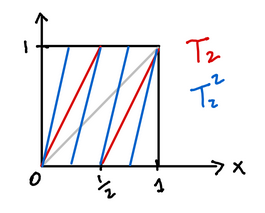
\includegraphics[width=5cm]{Immagini/Bernoulli.png}
    \caption{Un tipo di grafico utile la mappa di Bernoulli. In grigio troviamo l'identit\`a, in rosso $T_2$ e in blu $T_2^2$.}
\end{figure}

\noindent Evidentemente l'unico punto fisso \`e $0$ (dal disegno sarebbero $0$ e $1$, ma $0\equiv 1\mod 1$).\\
Cerchiamo ora punti con periodo minimo $2$, cio\`e
\[T^2(x)=x,\quad T(x)\neq x.\]
Ricordiamo che
\[T(x)=\begin{cases}
2x & 0\leq x< \frac12\\
2x-1 & \frac12\leq x<1
\end{cases}\implies
T^2=\begin{cases}
4x & 0\leq x<\frac14\\
2(2x)-1=4x-1 & \frac14\leq x<\frac12\\
2(2x-1)=4x-2 & \frac12\leq x<\frac34\\
2(2x-1)-1=4x-3 & \frac34\leq x<1
\end{cases}\]
Graficamente vediamo che ci sono due punti di periodo $2$, e questi sono $\frac13$ e $\frac23$. Osserviamo che i numeri della forma $3\ii\cdot 2^{-k}$ sono definitivamente periodici.\\
Cerchiamo i punti di periodo minimo $3$. Graficamente notiamo che sono $6$
    
\begin{figure}[!htb]
    \centering
    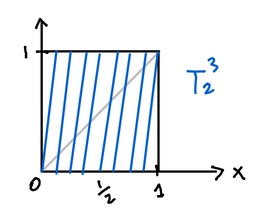
\includegraphics[width=5cm]{Immagini/Bernoulli_iterata.png}
    \caption{Rappresentazione grafica di $T^3_2$.}
\end{figure}

\noindent
In generale per come funzionano le iterate di $T_2$ si ha che il numero di punti di periodo (eventualmente non minimo) $n$ \`e $2^n-1$.
\end{example}

\begin{example}[Perdo il controllo]
Consideriamo la mappa
\[T:\funcDef{S^1}{S^1}{x}{10x \mod 1}.\]
Poniamo $\Ac=\cpa{0,\cdots,9}$ e $\Ac_n=\pa{\frac n{10},\frac{n+1}{10}}$ per $n\in\Ac$.\\
Sia $x\in \R\bs \Q$ e diamo la seguente mappa
\[\vp:x\mapsto(\omega_0,\omega_1,\cdots)\in \Ac^{\N}\]
dove $\omega_n=k\coimplies T^n(x)\in \Ac_k\coimplies \lfloor10 T^n(x)\rfloor=k$ e per ricorsione vediamo che $\omega_n$ \`e la $n$-esima cifra decimale di $x$, cio\`e
\[x=0.\omega_0\omega_1\omega_2\cdots.\]
Per rispondere ad una domanda del tipo ``$T^{1000}(x)\in \Ac_i?$" devo sapere la 1000-esima cifra di $x$. Se ora considero $x+\e$ al posto di $x$, le informazioni che avevamo su $x$ non dicono pi\`u nulla sul comportamento di $x+\e$ oltre un certo passo\footnote{se $i>-\log_{10} \e$ la risposta a ``$T^{1000}(x)\in \Ac_i?$" e quella a ``$T^{1000}(x+\e)\in \Ac_i?$" sono indipendenti.}.
\end{example}
    
\begin{remark}[Piccola parentesi statistica]
Sia $x=0.x_1x_2\cdots$ potremmo chiederci, fissata una cifra $k$ se
\[Prob\cpa{\lim_{N\to+\infty}\frac{\#\cpa{i\in \cpa{0,\cdots, N-1}\mid x_i=k}}{N}=\frac1{10}}=1\]
ed effettivamente \`e vero. Segue dunque che
\[Prob\cpa{\lim_{N\to+\infty}\frac{\#\cpa{i\in \cpa{0,\cdots, N-1}\mid x_i=k}}{N}=\frac1{9}}=0\]
anche se non \`e un insieme vuoto\footnote{per esempio posso fissare ogni nona cifra a $k$ e completare le altre con cifre a caso diverse da $k$.}.
\end{remark}

\begin{example}[Espansione binaria tramite la mappa di Bernoulli]
Sia $T_2:S^1\to S^1$, $T_2(x)=2x\mod 1$.\\
Sia $I_0=[0,\frac12)$, $I_1=[\frac12,1)$ e $\Omega=\cpa{0,1}^\N$. Consideriamo la mappa $\vp:S^1\to \Omega$ data da:
\[x\mapsto (\omega_0(x),\omega_1(x),\cdots),\quad \omega_i(x)=\begin{cases}
0 & T^i(x)\leq \frac12\\
1 & T^i(x)\geq\frac12
\end{cases}\]
Osserviamo che $\sigma\circ \vp=\vp\circ T_2$ ma $\vp$ non \`e un omeomorfismo (o ben definita), infatti
\[\vp\ii(1,0,0,0,\cdots)=\cpa{\frac12}=\vp\ii(0,1,1,1,1,\cdots).\]
Quello che sta succedendo che abbiamo trovato due serie della seguente forma che convergono allo stesso valore
\[x=\sum_{i\geq 0}\frac{\omega_i(x)}{2^{i+1}}.\]
    
\end{example}


\section{Mappa Logistica e Tenda}    
\begin{definition}[Mappa logistica]
Una funzione continua $T_\la:[0,1]\to[0,1]$ si dice \textbf{logistica} se \`e della forma
\[T_\la(x)=\la x(1-x),\quad 0\leq \la\leq 4.\]
\end{definition}
\begin{remark}
Le restrizioni $0\leq \la\leq 4$ servono per garantire che effettivamente $[0,1]$ sia il codominio.
\end{remark}

\begin{figure}[!htb]
    \centering
    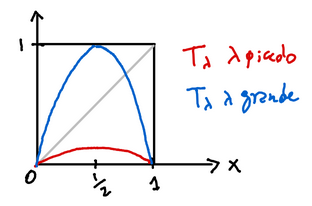
\includegraphics[width=6cm]{Immagini/Logistica.png}
    \caption{Rappresentazione di due mappe logistiche.}
\end{figure}


\begin{example}[Mappa logistica]
Osserviamo che $T_\la$ ha un massimo in $\frac12$.\\
Cerchiamo i punti fissi:
\[\la x(1-x)=x\coimplies x((\la-1)-\la x)=0,\]
quindi i punti fissi sono $0$ e $1-\la\ii$, dove il secondo punto fisso si presenta solo se compreso tra $0$ e $1$, cio\`e solo se $\la\geq 1$.
\end{example}
\begin{definition}[Mappa tenda]
Una funzione continua $T_s:[0,1]\to[0,1]$ si dice \textbf{tenda} se \`e della forma
\[T_s(x)=\begin{cases}
sx & 0\leq x< \frac12\\
s(1-x) & \frac12\leq x\leq 1
\end{cases},\quad 0\leq s\leq 2.\]
\end{definition}
    
\begin{remark}[Esempio di coniugio topologico]
La mappa logistica $T_4$ \`e coniugata topologicamente alla mappa tenda $T_2$.
\end{remark}
\begin{proof}
Basta considerare $\vp:[0,1]\to [0,1]$ data da
\[\vp(x)=\sin^2\pa{\frac\pi2x}\]
e notare che $\vp\circ T_2=T_4\circ \vp$\footnote{entrambe le composizioni assumono il valore $\sin^2(\pi x)$. Ricordiamo che $2\sin(\theta)\cos(\theta)=\sin(2\theta)$.}.
\end{proof}

\section{Sistemi caotici}
\begin{example}[Oscillatore armonico perturbato]
Sia $f:\R\to \R$ una funzione $1$-periodica. Immaginiamo una palla che rimbalza su un piatto la cui altezza varia come $f$. Per semplificarci la vita possiamo immaginare che l'urto avvenga sempre in $x=0$, tanto l'unica cosa che conta \`e $\dot f$ (l'impulso). Siano $t_0,t_1,\cdots,t_n$ i tempi di urto ($t_0=0$) e siano $v_0,\cdots,v_n$ le velocit\`a dopo l'urto. Conoscendo questi dati possiamo ricostruire tutta la dinamica.
\[T:\funcDef{[0,+\infty)\times (0,+\infty)}{[0,+\infty)\times (0,+\infty)}{(t_{n},v_n)}{(t_{n+1},v_{n+1})}.\]
Calcoliamo
\[\begin{cases}
t_{n+1}=t_n+h(v_n)\\
v_{n+1}=v_n+2\dot f(t_{n+1})
\end{cases},\quad h(v_n)=\frac 2gv_n\]
Osserviamo inoltre che
\[T(t_n+1,v_n)=(t_n+1+h(v_n), v_n+2\dot f(t_n+1 h(v_{n+1})))=T(t_n,v_n)+(1,0),\]
quindi in realt\`a possiamo considerare $S^1$ al posto di $[0,+\infty)$ per i tempi.\\
Questo sistema \`e difficile da trattare e presenta molti problemi aperti.
\end{example}
